\chapter{Introduction}\label{CH:introduction}

%******* WHY DONT YOU START INTRODUCING SURFACE TENSION HERE? TALK ABOUT ITS IMPORTANCE FOR ACUURATELY MODELING FLOWS*******

The study of fluid dynamics covers a wide array of phenomena across large spans of scales. Current research can be found exploring everything from biomedical simulations of capillary flows~\cite{biomed} to astrophysical approximations of star formations~\cite{star}. Researchers are studying bio-inspired dynamics of animals to gain insight into efficiency shortcomings of man made vessels~\cite{fish}. Other research focuses on oceanic current modeling to gain a deeper understanding of the natural world~\cite{ocean}. The focus of this research however, is on multiphase flows. In the context of this research, interest is restricted to flows where both a liquid and gas are present. These flows are referred to as gas-liquid flows, multiphase flows, or free surface flows in literature~\cite{gasliq,freesurf,brian}. Examples of gas-liquid flows can be seen throughout the natural world as well as industrial application and may be some of the most wide spread and common flow types on Earth. Bubbles rising in a carbonated drink, rain falling through the air, paint exiting a can of spray paint, a wave on the surface of the ocean; these are all examples of gas-liquid multiphase flows. These types of flows are of particular academic interest due to the ubiquity with which they emerge in industrial and engineering applications. For example, the increasing efficiency of internal combustion engines over the past several decades can largely be attributed to an increased understanding of the physics at work during fuel combustion. For efficient combustion to occur in a gasoline engine the fuel must first be atomized. Atomization is the process by which the fuel is broken from a stream into a fine mist or distribution of smaller droplets.


For engineering applications there are two main pathways by which multiphase flows are studied. Experimentation is a common method of study inside many scientific disciplines; the field of fluid dynamics is no different. Many researchers design experimental studies to gain deeper insight into the behavior of multiphase flows. Some examples of experimental techniques include shadowgraphy, x-ray imaging, or Particle image velocimetry (PIV)~\cite{shadow,piv,xray}. Computational fluid dynamics (CFD) is the second avenue used in multiphase flow study and is the focus this research.  CFD employs the computational power of modern computing to digitally investigate fluid flow problems. 


Within the field of CFD, simulation models are often classified by the scale to which they resolve turbulent structures. However, these methods all share the commonality that in some form or another, they all solve the Navier-Stokes equations which govern fluid flow. While many approaches exist, there are three main schemes: Reynolds Averaged Navier-Stokes (RANS), Large Eddy Simulation (LES), and Direct Numerical Simulation (DNS). These methods scale in fidelity respectively. RANS methods solve the time averaged Navier-Stokes equations. This is the least computationally intense method fo the three but requires a modeling scheme for all turbulent structures. Due to its low computational cost, RANS models are most commonly seen in industry application where a rough approximation of the turbulence scale is sufficient for design purposes. LES models are more computationally expensive than RANS models but are still fairly common in industrial engineering applications as well as academic research. LES methods solve filtered Navier-Stokes equations. This means that a filter is applied to the governing equations and then a closure model allows for the numerical simulation of the equations. The filtering operation and subsequent closure models give LES methods the ability to resolve some larger turbulent structures within a flow. While DNS methods are the most expensive of the three, they have the advantage of providing the most complete solution of the mathematical model. This is because direct simulations resolve the entire range of turbulent scales with no modeling necessary. Due to the computational expense however, DNS methods are usually reserved for academic interests in which a critical understanding of the realistic flow characteristics is required. An example of a simulated atomizing jet can be seen in Figure \ref{fig:DNSjet}. The image in this figure was produced from a DNS simulation. DNS methodology is the focus of this research. 

\begin{figure}[htbp]
	\centering
	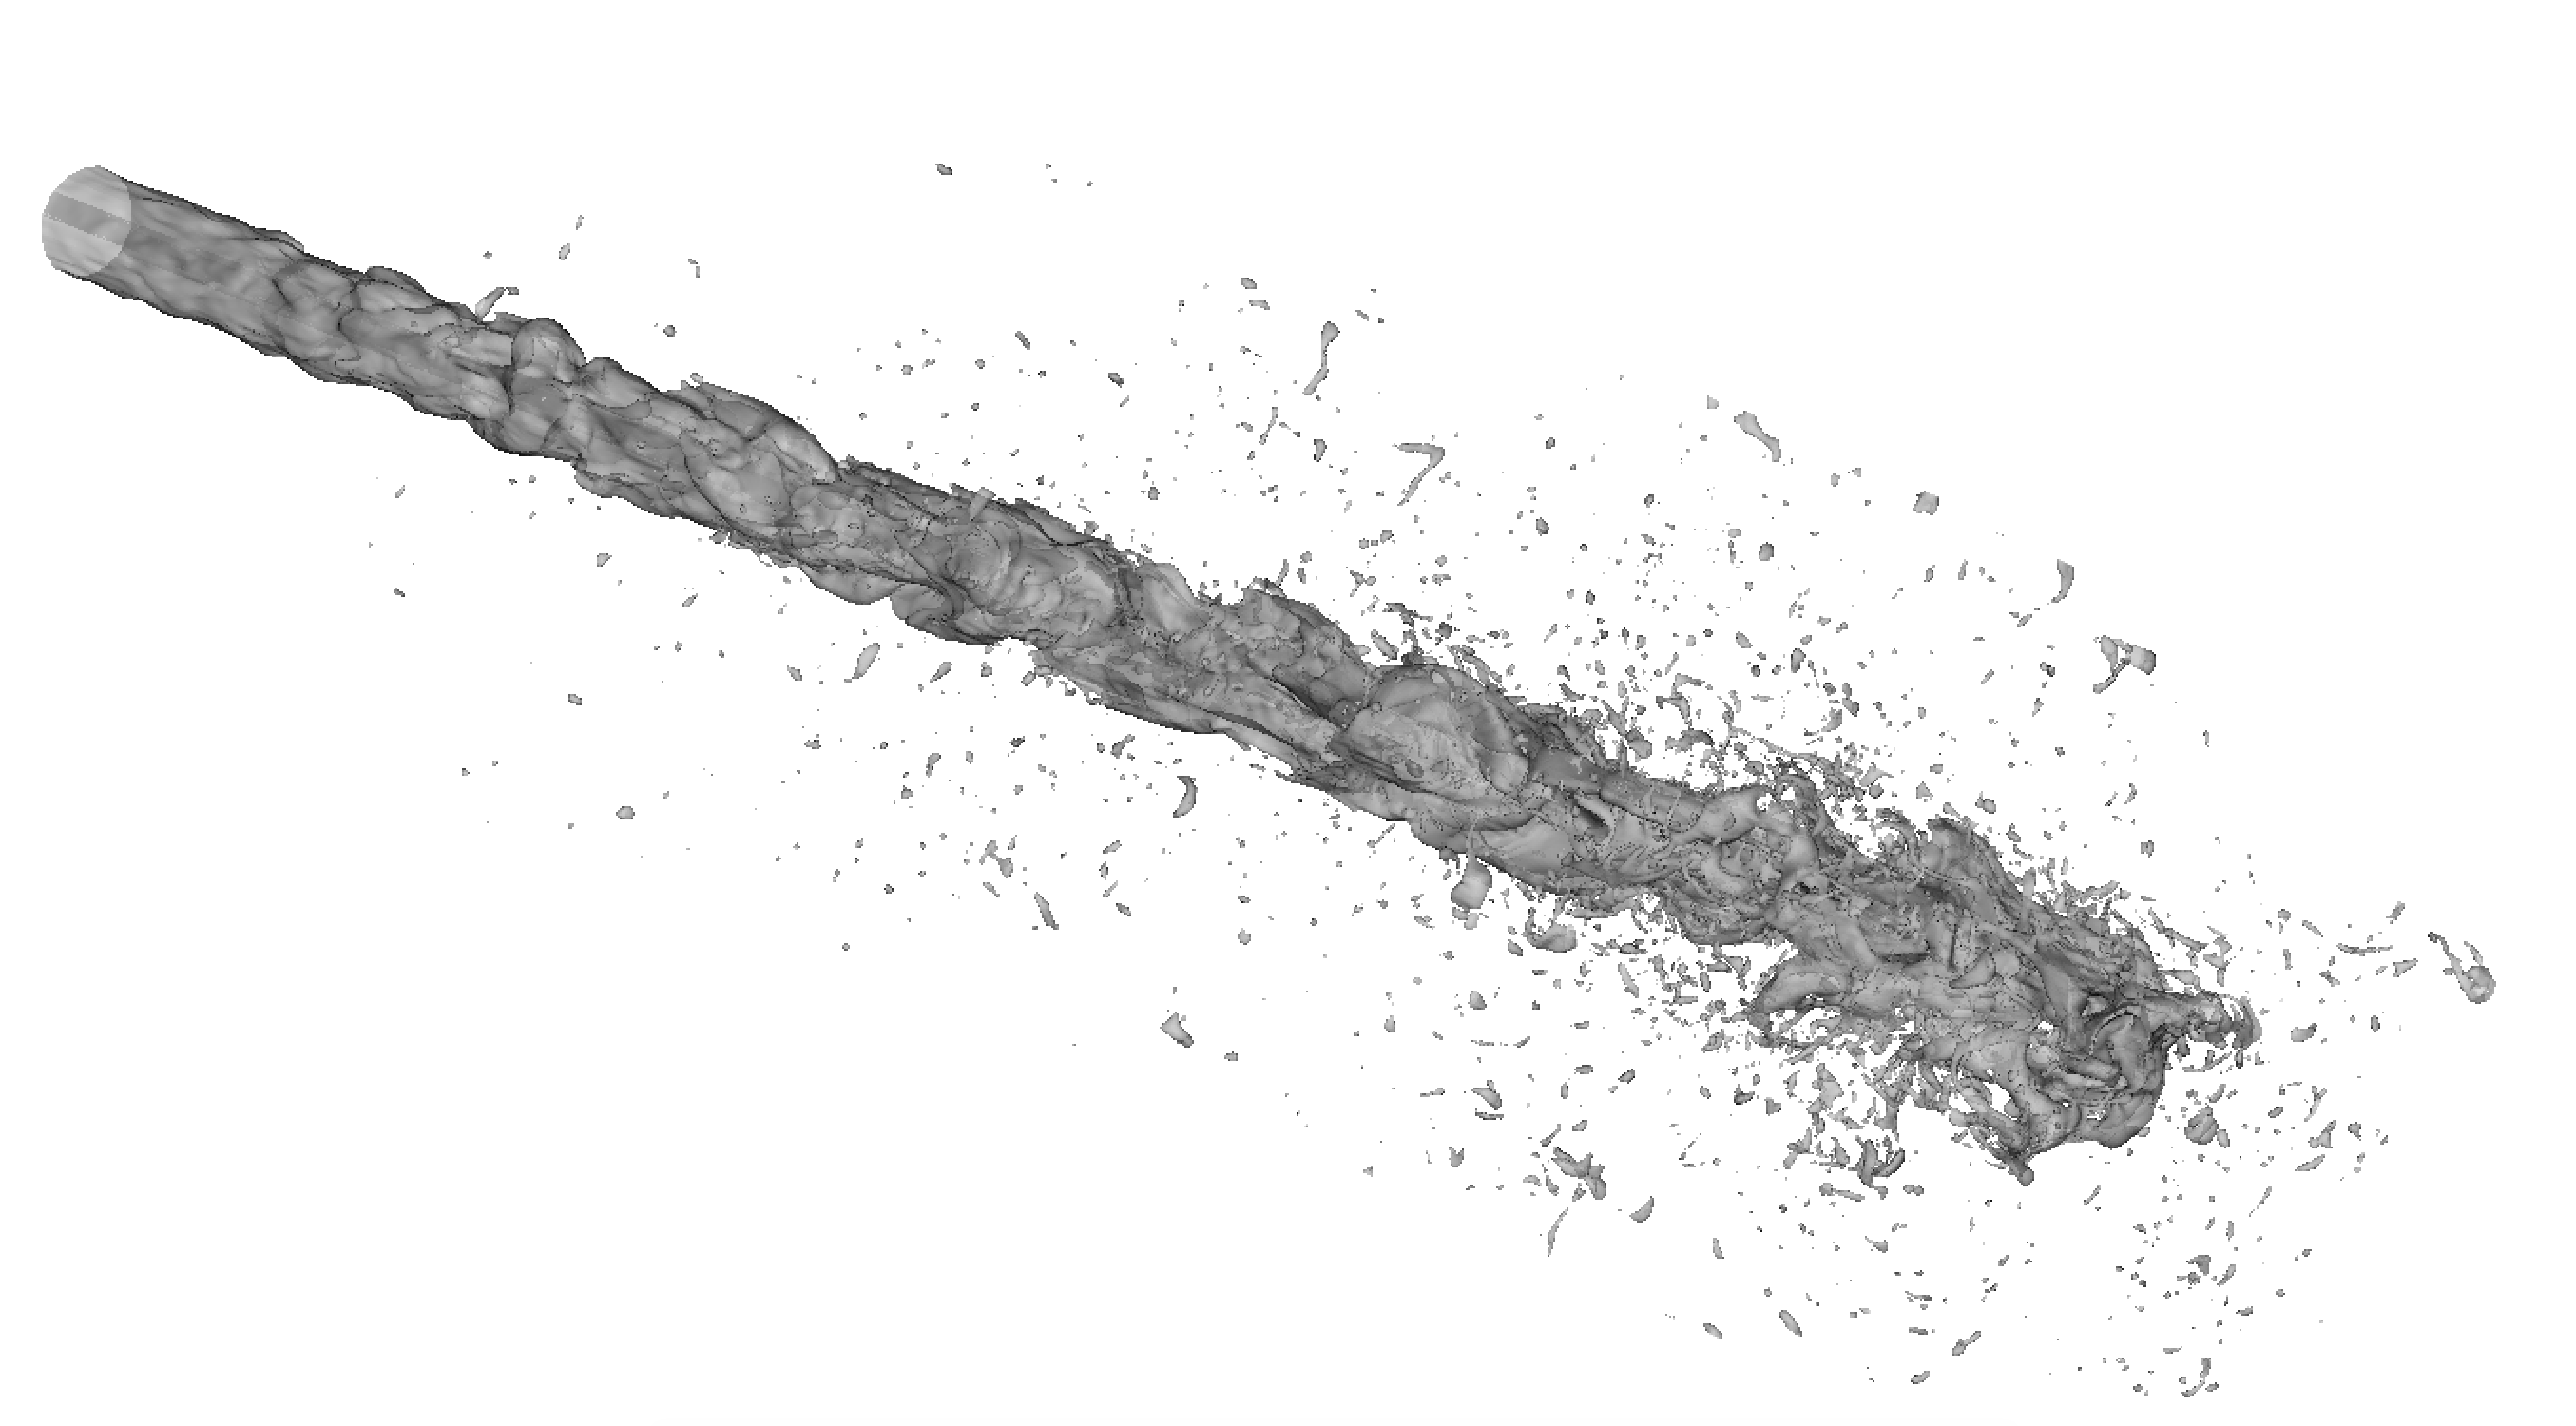
\includegraphics[width=0.8\textwidth]{figs/ACESjet}
	\caption{DNS Simulation of Atomizing Jet}
	\label{fig:DNSjet}
\end{figure}

Those involved in research using CFD can be segregated into two groups based on their research focus. Simulation based research utilizes in-house or commercial software packages to answer specific questions about fluid flow. An example of this might be a researcher trying to optimize an airfoil shape for specific flight conditions. With any number of software packages, various shapes and flow conditions can be simulated to determine an optimal geometry. Numerical methods for fluid dynamics focus on the accurate and efficient implementation of the Navier-Stokes equations, the governing equations of fluid mechanics, into numerical algorithms. An example of this might be the development of a new, more computationally efficient, method for solving partial differential equations. The focus of the research presented in this paper falls into this category. 

Numerous challenges exist concerning numerical methods of multiphase flows. One challenge of particular interest is the accurate representation of the intersection of the two fluids which exists for all gas-liquid multiphase flows. This intersection, known as the gas-liquid interface, presents notable challenge because the transition from one phase to another is represented as a mathematical discontinuity. That is, the change in density of the two fluids at the interface, is decidedly difficult to approximate mathematically. Surface tension is the governing force controlling the shape and behavior of the interface. For constant surface tension, the surface force($\textbf{f}_{\sigma}$) is expressed as $\textbf{f}_{\sigma} = \sigma \kappa \textbf{n}$\cite{Desjardins2013}. Here, $\sigma$ is given as the surface tension coefficient, a value empirically determined for all fluids. The vector perpendicular to the interface is \textbf{n}. The curvature of the interface is given by $\kappa$. Various curvature estimation schemes exist. Review of the mechanics which are required for this estimation along with a novel curvature scheme are the focus of the research to be discussed in the remainder of this work.    

 
%Stuff taken from past paper

%	Numerical models of surface tension play an important role in accurately predicting the behavior of multiphase flows such as those seen in the atomization process. Interface curvature is directly proportional to the surface tension force and controls many of the dynamics of an atomizing jet. Therefore, an accurate curvature calculation is vital for realistic analysis.  Height function methods (HFM) are a popular way of computing interface curvature in volume-of-fluid (VoF) architectures and were first introduced in the context of two-phase flows by Sussman~\cite{Sussman2003}. Standard height function methods, as seen in Fig.~\ref{fig:HFM}, calculate interfacial curvature by applying finite difference operators to heights which neighbor a cell of interest.


%\begin{figure}[h]

%	\begin{center}

%		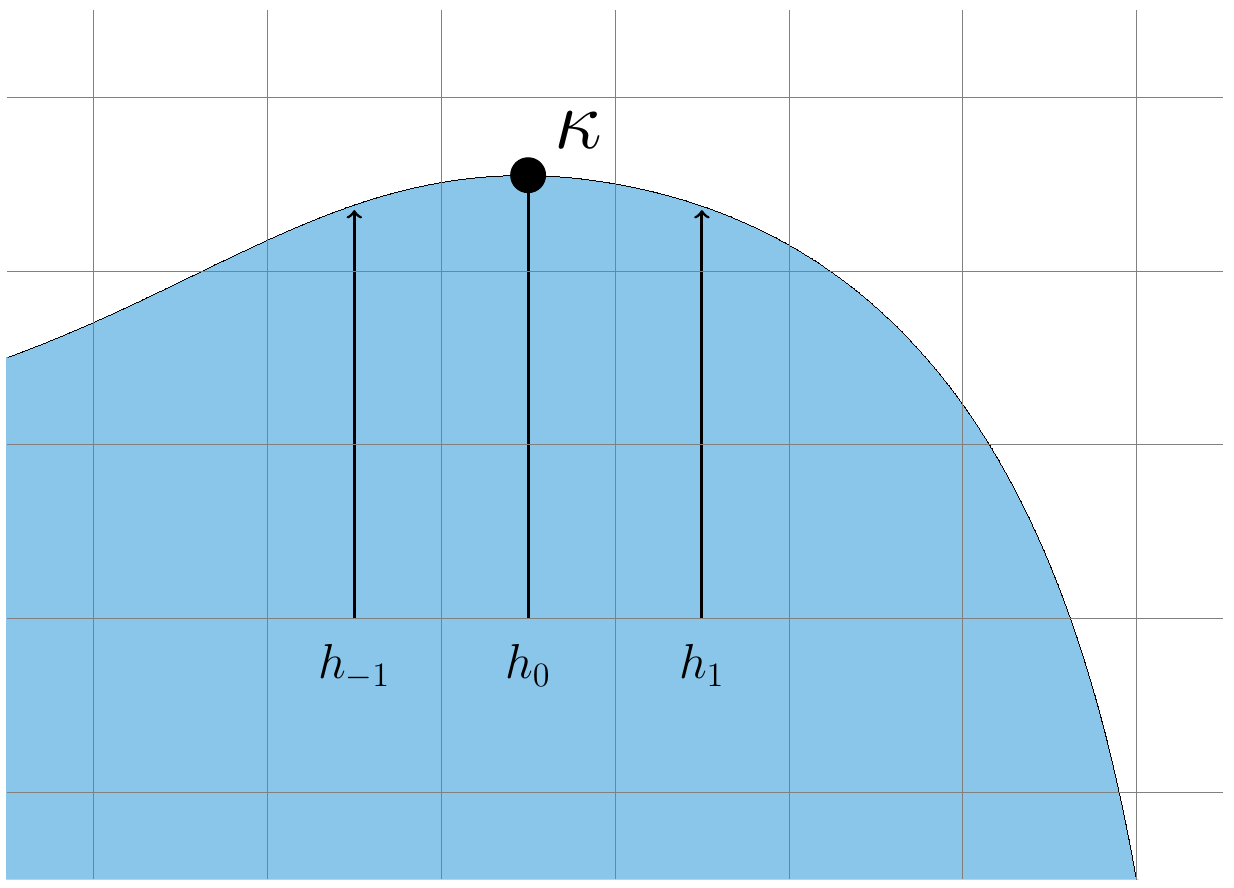
\includegraphics[width=2.5in]{figs/HFM.png}

%	\end{center}

%	\caption{Standard height function.}

%	\label{fig:HFM}

%\end{figure}


%Traditional mesh configurations calculate density at cell centers and momentum at cell faces. This can allow for an uncoupling of mass and momentum advection. Using a Rudman dual grid, which discretizes density on a twice as fine mesh, provides consistent and conservative discretizations by calculating fluxes on sub-faces~\cite{Rudman1998}. However when a dual grid is used, the standard height function method fails to capture fine grid interface perturbations. 	These perturbations can grow uncontrollably and result in non-physical dynamics occurring in simulations. An example of tihs uncontrolled growth resulting in non-physical dynamics can be seen in Fig.~\ref{bad2}. This research develops an extension of the standard height function to include information from the Rudman dual mesh. This method results in consistent mass and momentum transport while also providing accurate interface transport that avoids non-physical dynamics.


